\documentclass[24pt]{beamer}

\usepackage[utf8]{inputenc}
\usepackage[T1]{fontenc}
\usepackage{graphicx}


\title{Themenvorschläge der Java-Gruppe}
\subtitle{Netzwerksimulator Sinalgo oder Neuronale Netze mit Neuroph}
\author{Markus Braun, Daniel Hammann,\\ 
	Dominik Messinger, Dominic Rausch}


\begin{document}
	\maketitle

	\begin{frame}[c]\frametitle{Sinalgo\footnote{http://disco.ethz.ch/projects/sinalgo/} }
		\begin{itemize}
			\item Netzwerksimulator von der ETH
			\item Features
			\begin{itemize}
				\item Bewegliche Knotenpunkte
				\item Eigenes Verbindungsmodel
				\item Eigenes Interferenz- und Verlässlichkeitsmodel
				\item Übertragungszeit
			\end{itemize}
			\item \textbf{Langsam!}
		\end{itemize}
	\end{frame}

	\begin{frame}[c]\frametitle{Sinalgo - Was ist zu tun?}
		\begin{itemize}
			\item Status Quo:
		    \begin{itemize}
		    	\item Ein Thread
		    	\item Mehrfache Iteration über jeden Knoten
		    	\item Asynchron und Synchron Modus
		    \end{itemize}
		    \item Herausforderungen:
		    \begin{itemize}
		    	\item Nebenläufiges Verschieben und Neuverbinden der Knoten
		    	\item Nebenläufige Simulation des Knotenverhaltens
		    	\item Evtl: Anpassung der GUI nötig
		    \end{itemize}
		\end{itemize}
	\end{frame}
	
	\begin{frame}[c]\frametitle{Neuroph\footnote{http://neuroph.sourceforge.net/}}
		\begin{itemize}
			\item Künstliches Neuronales Netz - Framework in Java
			\item Features
			\begin {itemize}
				\item leichtgewichtiges, intuitives Framework
				\item unterstützt verschiedene ANNs, z.B. Multi Layer Perzeptron mit Backpropagation
				\item Anwendungen sind Klassifikations-, Erkennungsaufgaben, Vorhersagen...
			\end {itemize}
			\item versteckte Schicht mit 500 Neuronen $\rightarrow$ \textbf{47s!!}
		\end {itemize}
		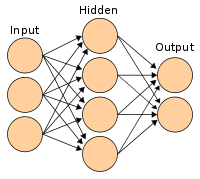
\includegraphics[scale=0.5]{ann.png}
	\end {frame}
	
	\begin{frame}[c]\frametitle{Neuroph - Was ist zu tun?}
		\begin{itemize}
			\item Status Quo:
		    \begin{itemize}
		    	\item Ein Thread pro komplettes Traning-Set
		    	\item MLP: Iteration über Layer, pro Layer wiederum Iteration über Neuronen
		    	\item große Schicht führt unmittelbar zu langer Laufzeit
		    \end{itemize}
		    \item Herausforderungen:
		    \begin{itemize}
		    	\item Nebenläufiges Trainieren und Anwenden: Schichten aufteilen und parallel berechnen
		    \end{itemize}
		\end{itemize}
	\end{frame}

\end{document}